\renewcommand{\theequation}{\theenumi}
\begin{enumerate}[label=\arabic*.,ref=\thesubsection.\theenumi]
\numberwithin{equation}{enumi}
\item no of total families chosen for survey = 2400
\\
No of families owning 2 vehicles and earning of \rupee 10000 - \rupee13000 per month = 1
\begin{align}
P\left(X=1\right) &= \frac{29}{2400}
&= 0.012
\end{align}
\\
\item No of families earning \rupee 16000 and more per month and owning exactly 1 vehicle = 579
\\
P(X=2) = probability of a family to have 1 vehicle with earning of \rupee 16000 and more 
\begin{align}
P\left(X=2\right) &= \frac{579}{2400}
\\
&= 0.241
\end{align}
\\
\item No of families earning  less than \rupee 7000  per month and owning exactly no vehicle = 10
\\
P(X=3) = probability of a family to have no vehicle with earning less than \rupee 7000  
\begin{align}
P\left(X=3\right) &= \frac{10}{2400}
\\
&= 0.0042
\end{align}
\item No of families earning   \rupee 13000  to \rupee 16000  per month and owning more than 2 vehicle = 25
\\
P(D) = probability of a family to have more than 2 vehicles with earning \rupee 13000 to \rupee 16000 per month   
\begin{align}
P\left(X=4\right) &= \frac{25}{2400}
\\
&= 0.0104
\end{align}
\item No of families owning not  more than 1 vehicle $\to$
\\
earning less than \rupee 7000 = 170
\\
earning \rupee 7000 to \rupee 10000 = 305
\\
earning \rupee 7000 to \rupee 10000 = 536
\\
earning \rupee 7000 to \rupee 10000 = 471
\\
earning \rupee 7000 to \rupee 10000 = 580
\\
total no of families  = 1892
\\
\\
P(X=5) = probability of a family to have not more than 1vehicle    
\begin{align}
P\left(X=5\right) &= \frac{1892}{2400}
\\
&= 0.78833
\end{align}
codes for the above equation can be get from here
\begin{lstlisting}
codes/prob/prob8.py
\end{lstlisting}
\begin{figure}[!ht]
	\centering
	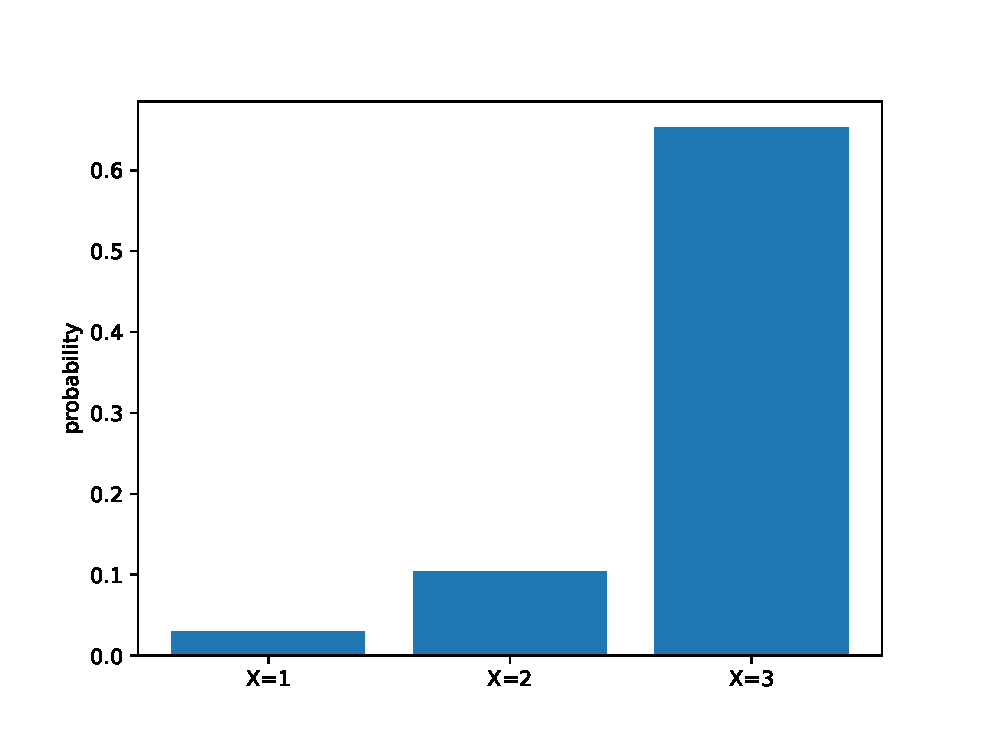
\includegraphics[width=\columnwidth]{./figures/probexm/probexm8.eps}
	\caption{probability of distance covered by tyre }
	\label{fig:bt8}
	\begin{lstlisting}
	figs/probexm/probexm8.eps
	\end{lstlisting}
\end{figure}
\end{enumerate}